\documentclass[a4paper,titlepage,12pt]{article}
\usepackage[utf8]{inputenc} %Make sure all UTF8 characters work in the document
\usepackage{graphicx}
\usepackage{titling}
\usepackage{tabularx}
\usepackage{longtable}
\usepackage[yyyymmdd]{datetime}
\usepackage[figurename=Figur]{caption}
\usepackage{booktabs}
\usepackage[parfill]{parskip}

%Set page size
\usepackage{geometry}
\geometry{margin=3cm}

\renewcommand{\dateseparator}{-}
\renewcommand{\contentsname}{Innehållsförteckning}
\renewcommand{\tablename}{Tabell}

%%%%%%%%%%%%%%%%%%%%%%%%%%%%%%%
% Header and footer
%%%%%%%%%%%%%%%%%%%%%%%%%%%%%%%
\usepackage{fancyhdr}
\pagestyle{fancy}

\lhead{
\includegraphics[width=0.15\linewidth]{../images/logo_full.png}}
\chead{Designspecifikation för sexbent robot}
\rhead{\today}
\setlength\headheight{26pt} 

\lfoot{TSEA29 -- KMM \\ LIPS Designspecifikation}
\rfoot{Grupp 9 \\ LiTHe Hex}

\newcommand{\itc}{I\textsuperscript{2}C}

\pretitle{%
	\begin{center}
		\LARGE
		
\includegraphics[width=6cm]{../images/logo_full.png}\\[\bigskipamount]
}

\posttitle{\end{center}}

\begin{document}
	\title{\LARGE
		\textbf{Designspecifikation för sexbent robot} \\
		\vspace*{0.5\baselineskip}
		\large
		Redaktör Frans Skarman \\
		Grupp 9 \\
		\small
		\vspace*{0.5\baselineskip}
		Version 0.1}

	\date{\today}

	\maketitle
	
	\newpage
	
	\begin{center}

		%%%%%%%%%%%%%%%%%%%%%%%%%%%%%%%%%%%%%%%%%%%%%%%%%%%%%%%%%%%%%%%%%%%%%%%%%%%%%%%%%
		%						Medlemmar
		%%%%%%%%%%%%%%%%%%%%%%%%%%%%%%%%%%%%%%%%%%%%%%%%%%%%%%%%%%%%%%%%%%%%%%%%%%%%%%%%%

		\section*{Projektidentitet}
		Grupp 9, Ht 2016, LiTHe Hex

		Linköpings Tekniska Högskola, ISY

		\renewcommand*{\arraystretch}{1.4}
		\begin{longtable}[c]{ l l l }
			\textbf{Namn} & \textbf{Ansvar} & \textbf{E-post} \\ \midrule
			Emil Segerbäck & & emise935@student.liu.se \\ \midrule
			Frans Skarman & Dokumentansvarig & frask812@student.liu.se \\ \midrule
			Hannes Tuhkala & & hantu447@student.liu.se \\ \midrule
			Malcolm Vigren & Projektledare & malvi108@student.liu.se \\ \midrule
			Noak Ringman &  & noari093@student.liu.se \\ \midrule
			Olav Övrebö &  & olaov121@student.liu.se \\ \midrule
			Robin Sliwa &  & robsl733@student.liu.se \\
		\end{longtable}

		\centering
		\textbf{Kursansvarig}: Tomas Svensson Rum 3B:528 013--28 13 68 tomas.svensson@liu.se

		\newpage
		\tableofcontents
		\newpage


		%%%%%%%%%%%%%%%%%%%%%%%%%%%%%%%%%%%%%%%%%%%%%%%%%%%%%%%%%%%%%%%%%%%%%%%%%%%%%%%%%
		%						Historik
		%%%%%%%%%%%%%%%%%%%%%%%%%%%%%%%%%%%%%%%%%%%%%%%%%%%%%%%%%%%%%%%%%%%%%%%%%%%%%%%%%

		\section*{Dokumenthistorik}
		\renewcommand*{\arraystretch}{1.4}
		\begin{longtable}[c]{ l l l l l }
			\textbf{Version} & \textbf{Datum} & \textbf{Utförda förändringar} 
			& \textbf{Utförda av} & \textbf{Granskad} \\ \midrule
			
			0.1 & 2016--??--?? & Första utkastet & Projektgruppen & \\
		\end{longtable}
	\end{center}

	%%%%%%%%%%%%%%%%%%%%%%%%%%%%%%%%%%%%%%%%%%%%%%%%%%%%%%%%%%%%%%%%%%%%%%%%%%%%%%%%%
	%						Inledning
	%%%%%%%%%%%%%%%%%%%%%%%%%%%%%%%%%%%%%%%%%%%%%%%%%%%%%%%%%%%%%%%%%%%%%%%%%%%%%%%%%

	\newpage

	\section{Inledning}
	I detta dokument beskrivs delsystemen för en sexbent robot mer ingående samt förslag på hur de ska 
	implementeras. De delsystem som roboten ska använda sig av är:
	Centralenhet, motorikenhet och sensorenhet.

	%%%%%%%%%%%%%%%%%%%%%%%%%%%%%%%%%%%%%%%%%%%%%%%%%%%%%%%%%%%%%%%%%%%%%%%%%%%%%%%%%
	%						Översikt
	%%%%%%%%%%%%%%%%%%%%%%%%%%%%%%%%%%%%%%%%%%%%%%%%%%%%%%%%%%%%%%%%%%%%%%%%%%%%%%%%%

	\section{Systemöversikt}
	Systemet ska innehålla tre enheter. En centralenhet för kommunikation med en
	dator, en motorikenhet som sköter hur benen rör sig samt en sensorenhet som
	tolkar sensordata. Centralenheten är även den enhet som tar beslut och
	kommunicerar med de andra enheterna. Se Figur.~\ref{fig:overview} för en översiktsbild av
	systemet.
	\begin{figure}[h]
		\centering
		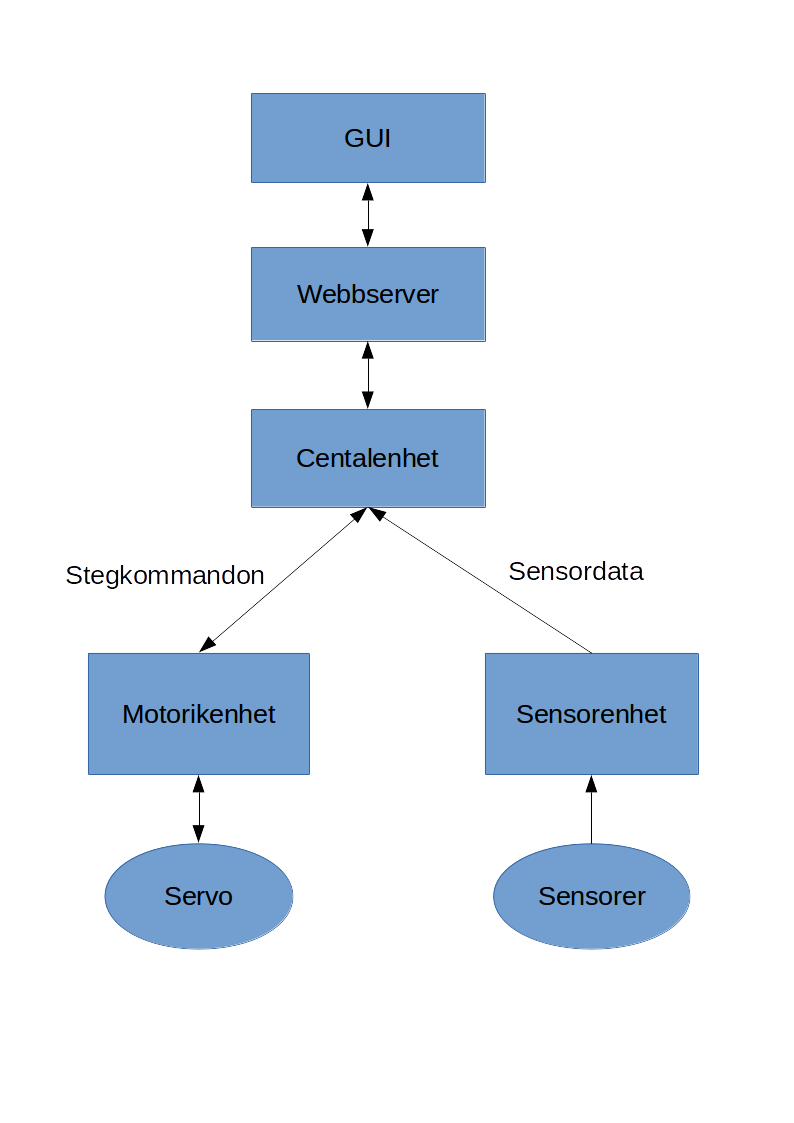
\includegraphics[width=0.5\linewidth]{../images/overview.png}
		\caption{Översikt av systemet\label{fig:overview}}
	\end{figure}

	\section{Komponentbudget} 
	Centralenhet 
	Raspberry Pi 3 
	Sensorenheten
	Atmega1284 
	GP2D120
	GP2Y0A02YK 5 stycken
	Lidar laser
	Resistorer 
	Kondensatorer 
	Motorikenheten 
	Atmega1284

	\subsection{Kommunikation mellan enheterna}
	Kommunikation mellan centralenheten och de två AVR-processorerna kommer att ske
	med SPI. Sensor- och motorikenhetens SPI portar kommer att kopplas till var sin
	SPI port på raspberry PI:en. Kommunikationen kommer huvudsakligen ske genom  att
	centralenheten begär data eller skickar kommandon till sub-enheterna som
	sedan svarar på begäran.  

	\subsubsection*{Kommunikationsprotokoll}
	\label{ssub:Kommunikationsprotokoll}
	Kommuikationen mellan centralenheten, motorikenheten och sensorenheten kommer att ske 
	med protokollet som beskrivs i figur \ref{fig:kommunikation1}

	\begin{figure}[h]
		\centering
		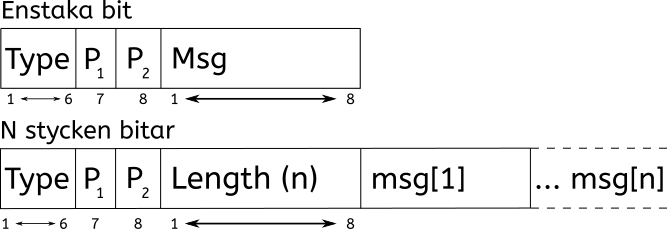
\includegraphics[width=0.5\linewidth]{images/communication_protocol1.png}
		\caption{Översiktlig vy av kommunikationsprotokolllet}
		\label{fig:kommunikation1}
	\end{figure}

	De första 6 bitarna av varje meddelande säger vilken typ av meddelande det är som
	skickas, de olika typer av meddelanden som kan skickas beskrivs i tabell 
	\ref{table:messages}. Den första biten i type parametern är 0 om meddelandets
	innehåll är en enstaka byte och 1 om meddelandet har dynamisk längd. Om längden
	är dynamisk är första biten i meddelanndet längden av resten.

	De två sista bitarna i första byten är paritetsbitar. Bit 7 är en  paritetsbit
	för meddelandets innehåll medan bit 8 är paritetsbit för de 7 tidigare bitarna.

	Om någon av paritetsbitarna är fel så kommer enheten som tog emot meddelandet att svara
	med ett speciellt meddelande för att indikera sändningsfel. Annars kommer den 
	att svara med ett 'acknowledge' meddelande.

	\begin{table}
		\begin{longtable}[c]{ l l l }
			\textbf{Syfte} & \textbf{ID} & \textbf{Data} \\ \midrule
			\textbf{Generella} \\ \midrule
			Send fail & 00 & -- \\ \midrule
			Acknowledge & 01 & -- \\ \midrule
			Datarequest & 02 & data \\ \midrule
			\\
			\textbf{Centralenhet $ \to $ motorikenhet}\\ \midrule
			Toggle hindergång & 03 & på/av \\ \midrule
			Sätt servohastighet & 04 & $ hastighet $ \\ \midrule
			Gåkommando &  20 & len, x-hastighet, y-hastighet, svänghastighet \\ \midrule
			Return to neutral & 05 & -- \\ \midrule
			\\
			\textbf{Centralenhet $ \gets $ motorikenhet}\\ \midrule
			Servostatus & 20 & len, ... data ... \\ \midrule
			Debugsträng & 21 & len, "debugsträng i utf-8" \\ \midrule
			Hinder här? & 03 & ja/nej \\ \midrule
			\\
			\textbf{Centralenhet $\to$ sensorenhet} \\ \midrule
			Återställ orientering & 03 & -- \\ \midrule
			\\
			\textbf{Centralenhet $ \gets $ sensorenhet}\\ \midrule
			Behandlad sensordata & 20 & len, ... avståndsmätardata ..., gyrodata \\ \midrule
			Korridordata		 & 21 & len, ... avstånd till väggar ..., vinkel \\
		\end{longtable}

		\vspace{0.5cm}
		\label{table:messages}
		\caption{Lista av meddelanden som kan skickas mellan enheter}
	\end{table}
	
	
	\section{Centralenheten}
	Centralenheten har tre ansvarsområden: navigation/beslutsfattning, hinderdetektion samt
	kommunikation med omvärlden.

	\subsection{Navigation och beslutsfattning}

	Centralenheten sköter all beslutsfattning om hur roboten ska röra sig
	genom labyrinten. Den tar emot data från sensorenheten och GUI:t och
	skickar kommandon till motorikenheten.
  
	\subsubsection{Autonomt läge}
	I det autonoma läget kommer entralenheten fråga om data från sensorenheten
    varje gång det ska fattas ett beslut. Detta gör att centralenheten själv
    bestämmer när den ska ha ny data för att den inte ska bli avbruten eller missa
    data för att den är mitt i utförandet av en annan funktion. Utifrån denna data
    fattar centralenheten beslut om hexapodens färdriktning.

    \subsubsection{Manuell navigation}
    För den manuella navigationen kommer sockets att användas mellan webbservern
    och centralenheten. Det kommer att komma in ett nytt meddelande med data för varje
    knapptryck/händelse som sker på GUIt som centralenheten tolkar och överför
    till motorikenheten. 
    % sockets används mellan centralenhet - server, server - client.

	\subsection{Hinderdetektion}
	%För hinderdetektering finns det olika alternativ att använda. Det är möjligt att 
	%detektera hinder med hjälp av en avståndsmätare som är vinklad nedåt, en IR-sensor 
	%eller LIDAR kan användas som avståndsmätare. Att använda en IR-sensor är fördelaktigt 
	%då IR-sensorer antagligen kommer att användas för att undvika väggar. En 
	%LIDAR är en ny enhet och medför ett ytterligare, mer avancerat gränssnitt. Ett annat 
	%alternativ för att upptäcka hinder är att läsa av det motstånd som benens servo kan 
	%returnera tillsammans med övriga sensorer för att upptäcka när roboten går in i ett 
	%hinder. 
	Sensorenheten har en avståndsmätare som är riktad snett neråt för att hitta kanten 
	på hinder. En IR-sensor används som avståndssensor. Vi kommer redan ha  kod för kommunikation med
	den  eftersom att IR-sensorer kommer att användas på andra ställen i konstruktionen. 
	
	\subsection{Kommunikation}
	Centralenheten ska kommunicera med en dator över WiFi. Det är datorns webbläsare 
	som kommer att ansluta till centralenhetens webbserver, det blir då möjligt att
	via webbgränssnittet att styra roboten samt läsa av robotens loggar. Det finns
	flera gränssnitt att 
	använda för kommunikation mellan processorerna. Intressanta gränssnitt är SPI, 
	\itc{} och UART.\@ UART är inte möjligt att använda både till sensorenheten och 
	motorikenheten då Raspberry Pi endast har en UART-port. Både 
	SPI och \itc{} kan användas förutsett att LIDAR inte används. \itc{} måste konfigureras med ett
	master-/slave-förhållande. Centralenheten behöver vara master för att kunna
	kommunicera med 
	sensorenheten och motorikenheten som är slave. Med den konfigurationen blir 
	det inte möjligt för sensorenheten och motorikenheten att kommunicera med
	centralenheten utan att centralenheten har på startat kommunikationen. I och 
	med att \itc{} behöver en master/slave konfiguration blir SPI enklare att använda 
	för tvåvägskommunikation.
	
	% TODO: write more
	\subsubsection{Kommunikation med webbserver}
	Centralenheten kommunicerar med webbservern genom att skicka strängar med data till den. Strukturen på strängarna med data ser ut som ....

	%%%%%%%%%%%%%%%%%%%%%%%%%%%%%%%%%%%%%%%%%%%%%%%%%%%%%%%%%%%%%%%%%%%%%%%%%%%%%%%%%
	%						Motorikenheten
	%%%%%%%%%%%%%%%%%%%%%%%%%%%%%%%%%%%%%%%%%%%%%%%%%%%%%%%%%%%%%%%%%%%%%%%%%%%%%%%%%
	\section{Motorikenheten}
	Motorikenheten översätter kommandon från centralen till servokommandon. Den tar emot 
	instruktioner från centralenheten som anger hastighet, rotation och riktning för 
	förflyttnnig. Motorikenheten behandlar detta, räknar ut en lämplig gångstil och 
	signalerar nödvändiga vinklar till de sex benen. Vissa delmoment i förflyttningen 
	görs hårdkodade. 
	
		\subsection{Planläggning}
	Första steget i motorikenheten för en anpassad gångstil är att utifrån efterfrågad
	förflyttning avgöra en önskad slutposition för respektive ben, som för roboten närmre 
	ett läge indikerat av centralenheten. Utifrån hastighet skalas förflyttningsvektorerna 
	från nuvarande läge för varje ben ner. Benen flyttas i grupper av tre med ett pen på 
	ena sidan och två på  andra (uppdelat på ett mittenben, respektive ett framben och ett 
	bakben). När ett sett ben förflyttas, skiftas de markfästa benen vid behov för 
	att flytta själva kroppen, även denna utifrån en förflyttningsvektor (som med benen). 
	Lyft och nedsättning av ben hårdkodas, sådan att alla tre ben som skall flyttas i ett 
	sett höjs, och sänks först när de satts i önskad position, sådan att benens position 
	och förflyttning för vanlig gång kan beräknas i planet, snarare än i rummet, med 
	avseende på beslutsfattning. Endast vid den inverterade kinematiken krävs då 
	tredimensionell planering av benens rörelser. Detta beteende finns även illustrerat i 
	figur \ref{fig:walkflow0}. 
	
	För analog styrning ska hastighet även kunna anpassas genom justering av servonas
	hastighetsinställning.

	\begin{figure}[h]
		\centering
		\includegraphics[width=0.5\linewidth]{images/gangstil_flowchart.png}
		\caption{Flödesschema för normal gångstil hos roboten \label{fig:walkflow0}}
	\end{figure}

	\subsection{Hindergång}
	För hindergång ska roboten treva med benen, och anpassa sig efter höjdskilnaden genom
	läsning av benens mötta motstånd. Benen sänks till det att de möter motstånd, dels
	vid uppstegning på hindret, men också vid gång på hindret, för att upptäcka när hindret 
	tar slut. Inför uppgång på hinder höjs även benen extra, för att tillåta kliven att nå 
	upp till hindret.

	Därtill gäller att benen flyttas marginellt (någon centimeter) vid uppkliv på eller 
	nedkliv från hinder. Detta för att undvika att fötterna hamnar instabilt på kanten till 
	hindret, men roboten tycker sig ha stå stabilt, men även för att vid nedstig få en benen 
	länre fram, för att undvika att falla frammåt. En översikt över detta kan fås i figur \ref{fig:walkflow1}.

	\subsection{Inverterad kinematik}
	Då planläggningsdelen av motorikenheten beslutat om var ett ben skall flyttas beräknas 
	lämpliga vinklar för benets alla servon genom inverterad kinematik. Utifrån kända 
	längder på benen och positioner där man vill att fötterna ska placeras används 
	trigonometri och linjär algebra för att avgöra slutgiltiga servovinklar.

	\subsection{Kommunikation med servon}
	Servona styrs via en uart-länk, med hjälp av addresserade datapaket. Vid behov, 
	som vid justering av hastighet, ändras inställningarna i servona själva, allt 
	utifrån metoden beskriven i databladet för AX-12 servon.
	
	Då standardiserad baud rate för AX-12 är förhållandevis hög kan assembly-kod (via C) 
	användas för att justera denna till en mer lätthanterlig hastighet (med en instruktion
	om mass-skrivning till address 04 i servona, igen, enligt databladet).
	
	\begin{figure}[h!]
		\centering
		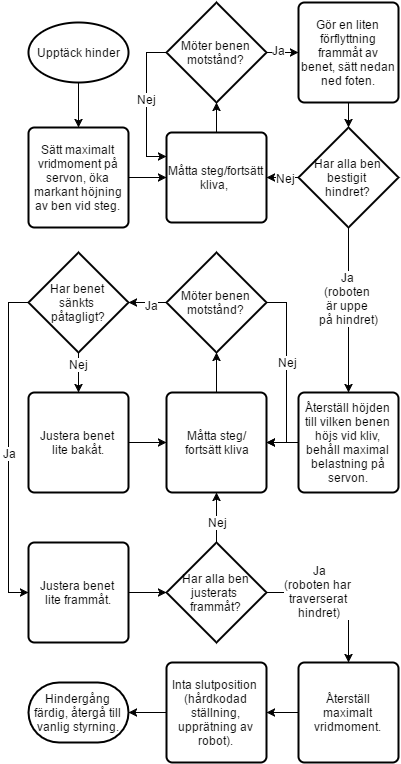
\includegraphics[width=0.5\linewidth]{images/hindergang_flowchart.png}
		\caption{Flödesschema för hindergångsprocedur hos roboten \label{fig:walkflow1}}
	\end{figure}
    
    \newpage

	%%%%%%%%%%%%%%%%%%%%%%%%%%%%%%%%%%%%%%%%%%%%%%%%%%%%%%%%%%%%%%%%%%%%%%%%%%%%%%%%%
	%						Sensorenheten
	%%%%%%%%%%%%%%%%%%%%%%%%%%%%%%%%%%%%%%%%%%%%%%%%%%%%%%%%%%%%%%%%%%%%%%%%%%%%%%%%%
	\section{Sensorenheten}
	
	Sensorenheten är den enhet som ger roboten sinnen för omvärlden, så att den
	kan navigera autonomt genom labyrinten. Sensorenheten ska för
	centralenheten vara ett abstrakt gränssnitt till sensorerna. Centralenheten
	behöver alltså inte veta exakt vilka sensorer som används, utan istället
	läser av data som "avstånd till vägg", eller "vridning relativt väggarna".

	\subsection{Styrenhet i sensorenheten}

	Styrenheten för sensorenheten ska bestå av AVR-processorn Atmega1284, som läser av och 
	behandlar informationen från robotens sensorer. Styrenheten sköter även
	kommunikationen med centralenheten -- den tar emot förfrågningar om data och
	skickar behandlad data på begäran.

	Styrenheten ska behandla den råa sensordatan till den grad att
	centralenheten inte behöver allt för mycket egna beräkningar på
	sensorinformationen. Den ska därför bland annat sköta brusreducering av
	datan, samt beräkna integralen av informationen från gyrot för att få ut en
	faktisk vinkel som roboten roterat. ATmega1284 kommer att ha tillräckligt med 
	beräkningskraft för att ta hand om den datan som sensorerna genererar. Den kritiska 
	delen är istället A/D-omvandling. Eftersom vi har många IR-sensorer tar det tid att 
	mäta och omvandla de analoga signalerna till digitala värden, en A/D omvandling kan ta 
	upp till 260 mikrosekunder. Om vi får problem med att IR-sensorerna interfererar med 
	varandra kan endast en IR-sensor mäta åtgången. Vid dessa omständigheter kan 
	centralenheten inte få nya värden 4 ggr/sec ens.

    \subsubsection{Huvudloop}
    Huvudloopen 

    Flödesschemat för den kod som är tänkt att köras kan ses i figur
    \ref{fig:sensor_flow}. 
	Datastrukturer:
	Kö -- En struktur för kö behövs för schema läggning av IR-sersorer. 
	IR -- En struktur som hanterar varje IR-sensor. 
    \newpage

    \begin{figure}[h!]
        \centering{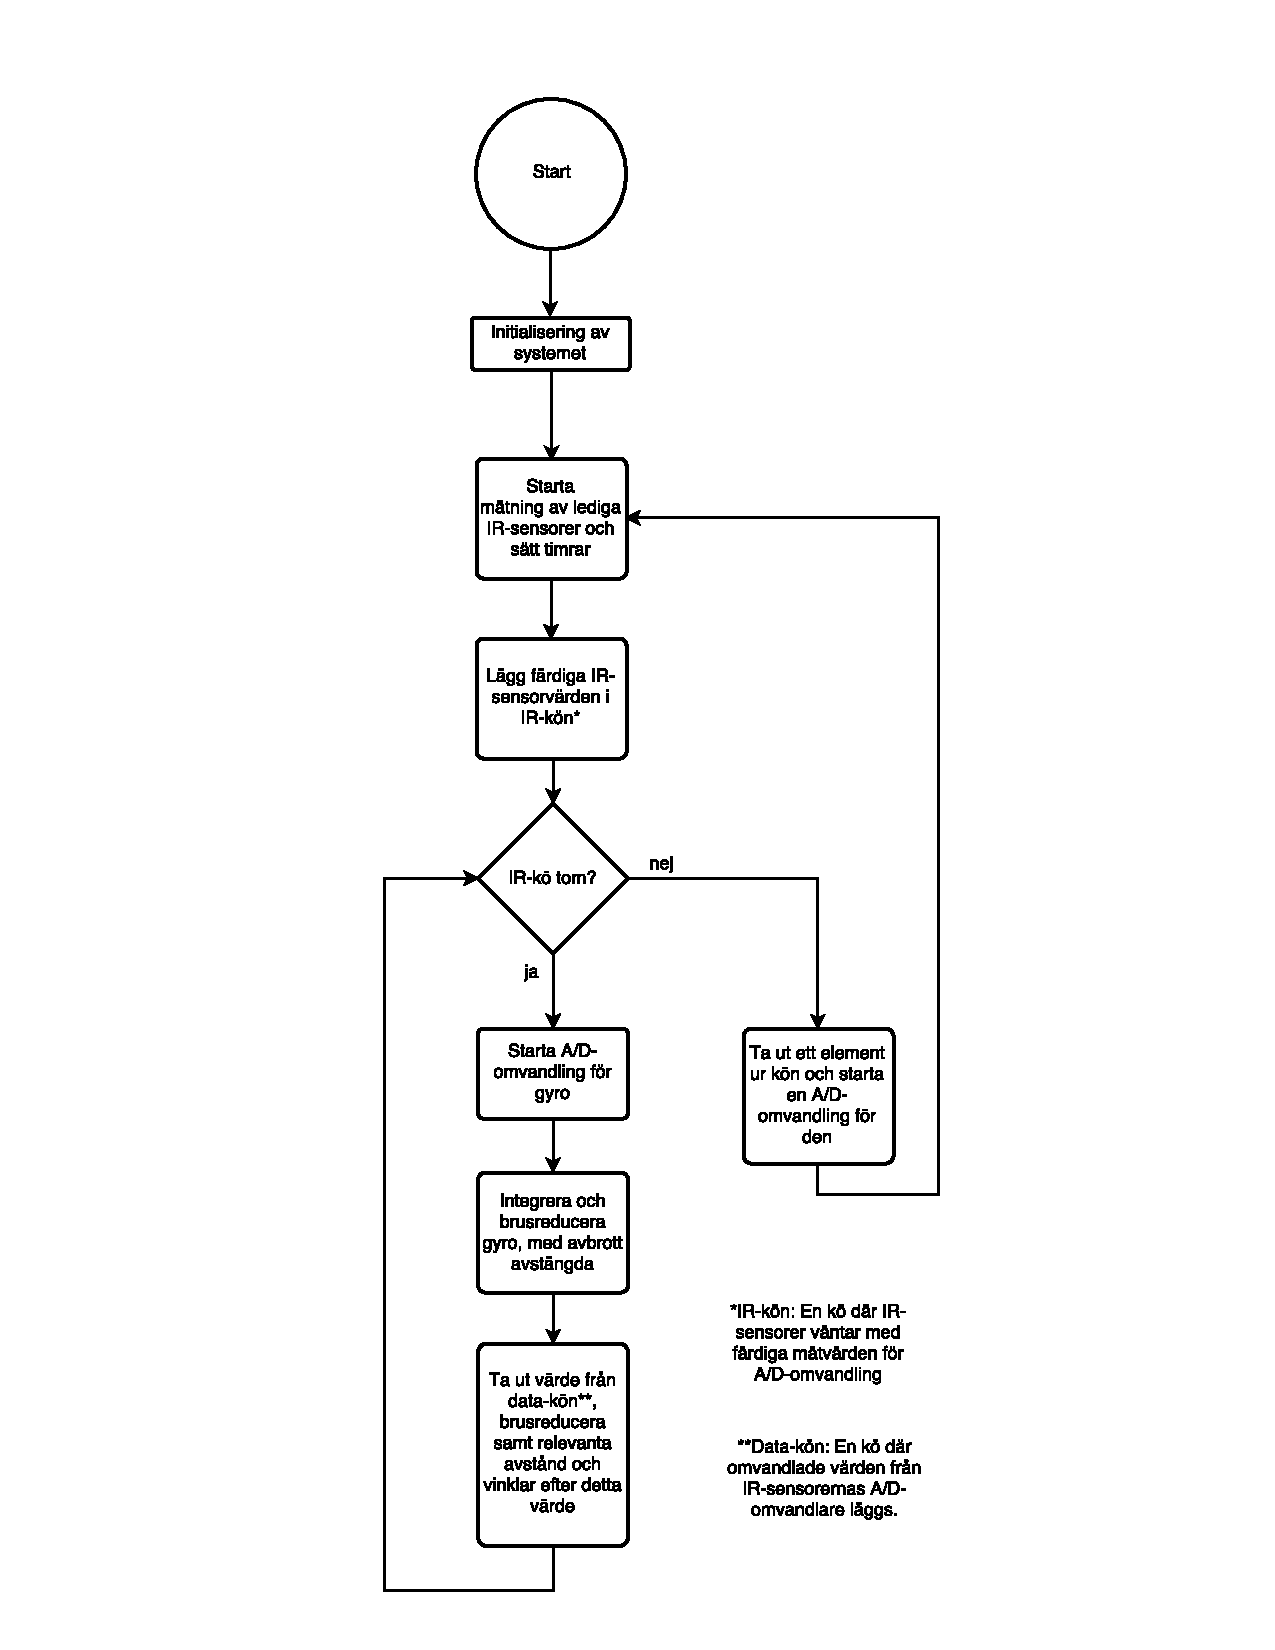
\includegraphics[width=17cm]{images/flowchart_sensor.pdf}}
        \caption{Flödeschema för huvudloopen\label{fig:sensor_flow}}
    \end{figure}

    \newpage

    \subsubsection{Avbrott}
	Följade avbrott kommer att vara aktiva:
    \begin{itemize}
        \item Avbrott 25 genereras när den interna A/D-omvandlaren är klar 
            vilket används för IR-sensorerna. När A/D-omvandlingen är klar 
            sparas värdet i en lista som behanlas vid ett senare tillfälle.
        \item Avbrott 20 genereras när någon bit i registret för SPI kommunikationen
            ändras. Det kommer att användas för kommunikationen över SPI där skicka och 
            ta emot data mellan sensorenheten och centralenheten. Avbrotts koden för 
            SPI kommer att vara ganska stor för att den ska kunna behandla flera olika fall.
        \item Avbrott 27 genereras när någon bit i registret för \itc{} kommunikationen 
            ändras. Bitarna kommer att ändras när data skickas och tas emot med LIDAR.
            Värdet från LIDAR sparas för att behandla senare.
    \end{itemize}

	%\\Avbrott 14 genereras när Counter1 blir lika med ett specikt värde. Kommer att användas när 
	%för att veta när IR-sensorer kan mäta. 
	%\\Avbrott 33 genereras när Counter3 blir lika med ett specikt värde. Kommer att användas när 
	%för att veta när Gyro kan mäta. 

    % \begin{table}[h!]
    %     \begin{center}
    %     \begin{tabular}{l l}
    %         \textbf{Avbrott} & \textbf{Funktion} \\ \hline 
    %         A/D-omvandling klar & Lägg färdig data i huvudtabellen \\ \hline
    %         SPI-meddelande mottagen & Tolka förfrågan och skicka SPI-meddelande
    %         som svar \\ \hline
    %         \itc{} & Läs LIDAR-sensorvärde, brusreducera och lägg
    %         i tabellen \\ 

    %     \end{tabular}
    %     \end{center}
    %     \caption{De avbrott som ska användas}
    % \end{table}


	%Program flöde:

	%Vänta 30 hundradelar för att allt ska starta och första mätvärdet från IR-sensorer blir 
	%klart. 

	%IR tabellen 5 stor --> gör brusred. 

	%Gyro tabellen 5 stor --> gör brusred.
	
	%LIDAR tabellen 5 stor --> gör brusred.

	

	%IR - IR analog blir digital(A/D), läggs i tabell, när tabell är 5 stor gör brusred., 
	%IR data klar att skickas till Centralenheten.
	
	%Gyro - Gyro digital integreras läggs i tabell, när tabell är X stor gör brusred., 
	%gyro data klar att skickas till Centralenheten. 

	%LIDAR - Digital läggs i tabell, när tabell är X stor gör brusred., 
	%LIDAR data klar att skickas till Centralenheten. 
	

	\subsection{Gyro}

	Sensorenheten ska använda ett gyro för att mäta vridning i det horisontella
	planet. Detta är användbart bland annat för att roboten ska veta hur mycket
	den ska rotera när den svänger. MLX90609 kommer att användas som gyro. Signalen från 
	MLX90609 läses analogt in till den interna A/D-omvandlaren på Atmega1284 som konverterar 
	den analoga signalen till ett digitalt värde med 10-bitars upplösning. 
	
	\subsection{Avståndssensorer fram}
	
	Sensorenheten ska använda avståndssensorer på framsidan, en sensor för att
	upptäcka väggar och en sensor som är snett vinklat ner mot golvet för hinderdetektion. 

	Avståndssensorn som mäter framåt ska utgöras av en LIDAR-sensor, som har
    ett mycket bredd mätspann (0-40m) med 1 centimeters upplösning.

	Sensorn som ska upptäcka hinder ska utgöras av en IR-sensor. Det
	har fördelen att ha samma gränssnitt som de andra IR-sensorerna som roboten
	ska använda.

	\subsection{Avståndssensorer åt sidorna}
	Roboten ska ha avståndssensorer på vardera långsida av roboten, för
	detektion av väggar och återvändsgränder. Dessa sensorer utgörs av 2
    IR-sensorer på varje sida där båda pekar ut från samma sida och
	är placerade på varsin ända av plattformen. Detta möjliggör mätning av hur
	roboten är vriden i en rak korridor och kan användas som felkontroll av
	gyrot.
	
	%%%%%%%%%%%%%%%%%%%%%%%%%%%%%%%%%%%%%%%%%%%%%%%%%%%%%%%%%%%%%%%%%%%%%%%%%%%%%%%%%
	%						Grafiskt användargränssnitt
	%%%%%%%%%%%%%%%%%%%%%%%%%%%%%%%%%%%%%%%%%%%%%%%%%%%%%%%%%%%%%%%%%%%%%%%%%%%%%%%%%
	%\newpage{}
	\section{Grafiskt användargränssnitt}
	På centralenheten ska en webbserver köras som tillhandahåller ett gränssnitt
	för användaren där man kan läsa sensordata eller kontrollera roboten i
	manuellt läge. Front-end-delen ska skrivas i Elm och back-end-delen i Elixir
    och webbramverket Phoenix.

	I det manuella läget ska roboten styras med en joystick som är kopplad till användarens
	dator eller med knappar på gränssnittet.
	
	\begin{figure}[h]
		\centering
		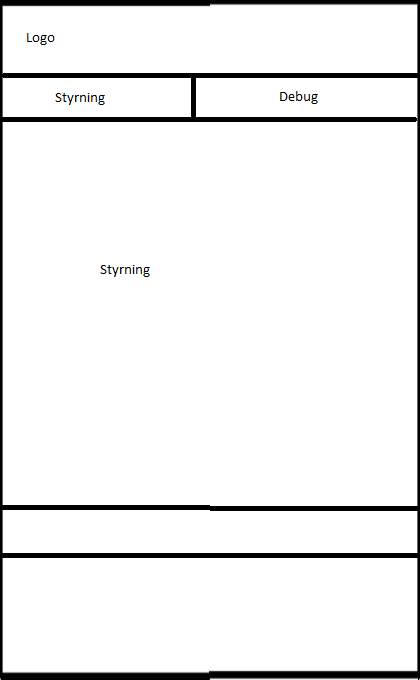
\includegraphics[width=0.5\linewidth]{images/gui-index.png}
		\caption{Figur av det grafiska gränssnittet\label{fig:gui-overview}}
	\end{figure}
    
    \subsection{Styrning}
    Under styrning ska man kunna styra roboten med en joystick. Man ska även
    kunna styra roboten med tangentbord eller knappar på skärmen. Det ska finnas
    en kryssruta som växlar mellan manuell och autonom styrning. För att styra
    roboten ska det finnas knappar som säger åt roboten att gå i en riktning,
    att vrida sig åt ett håll och att stanna.

    \subsection{Debug}
	Under debug ska robotens olika inställningars värden visas samt ska den visa all 
	sensordata vid tillfället. Var tredje sekund ska sidan uppdateras och klienten 
	hämtar den uppdaterade data:n med hjälp av JSON (Javascript Object Notation). 
	Det ska också finnas en eller flera grafer som beskriver några av de olika data.

	%%%%%%%%%%%%%%%%%%%%%%%%%%%%%%%%%%%%%%%%%%%%%%%%%%%%%%%%%%%%%%%%%%%%%%%%%%%%%%%%%
	%						Simuleringar
	%%%%%%%%%%%%%%%%%%%%%%%%%%%%%%%%%%%%%%%%%%%%%%%%%%%%%%%%%%%%%%%%%%%%%%%%%%%%%%%%%
	\section{Simuleringar}
	För att underlätta utvecklingen av vissa delar av projektet kommer vi att skriva
	kod för att simulera dessa delar. Simuleringarna ska kunna köra samma kod som ska
	köras på roboten men visualisera resultatet utan resten av roboten. De två
	delarna där simulering är mest aktuellt är inverterad kinematik, korridorföljning 
	och gångstil.

	% TODO: write more and correct it
	\subsection{Simulering för inverterad kinematik}
	Simuleringen går till genom en algoritm som går ut på att först räkna ut Jacobis matrisen för servornas position och dess vinkelräta enhetsvektor.
	
	Simuleringen kommer sedan att ritas ut med hjälp av algoritmen som beskrevs ovan i webbläsaren.
	
	\subsection{Simulering för korridorföljning}
	Simulering för korridorföljning kan testa olika regleralgoritmer utan att behöva testa 
	de på en gående robot. Simuleringen ritar ut en korridor och en robot som går framåt. 
	Simulatorn skickar ut sensorvärden till en fil, det är tänkta att regleralgoritmen ska 
	läsa in sensorvärden sedan ta beslut. Roboten i simulatorn använder 2 IR-sensorer på varje 
	sida som pekar rakt ut från roboten, det går att välja var på roboten som sensorerna ska 
	sitta. Beslutet av regleralgoritmen skrivs till en fil som simulatorn läser in och 
	styr roboten efter det. Det finns möjlighet att lägga till en störningsfunktion som till 
	exempel kan vara att roboten alltid går med en liten rotation. 
	
	\subsection{Simulering för gångstil}

\end{document}
